%% Contrôle recto-verso, deux compétences (Nature d'un angle, classer des angles).
%% Recto : Reconnaître la nature d'un angle ; verso : Classer des angles selon leur nature.
%% Réunit les anciens contrôles par compétence (un par face).
%% POUR LE CORRIGÉ : remplacer \corrigefalse par \corrigetrue (dans \begin{document}).

%% Font size %%
\documentclass[11pt]{article}

%% Load the custom package
\usepackage{Mathdoc}
\usepackage{colortbl}
\usetikzlibrary{calc}

%% Numéro de séquence %% Titre de la séquence %%
\renewcommand{\centerhead}{S04 - Éval : Nature d'un angle, classer des angles}

%% Spacing commands %%
\renewcommand{\baselinestretch}{1} \setlength{\parindent}{0pt}

% =================== Recto : Reconnaître la nature d'un angle ===================
% Corrigé : la feuille est écrite une seule fois (\feuille).
\newif\ifcorrige
% Réponse (texte) dans une case de largeur fixe : \rep[largeur]{réponse}
\newcommand{\rep}[2][1.6cm]{\makebox[#1]{\ifcorrige\textcolor{red}{\textbf{#2}}\else\dotfill\fi}}
% Mot à entourer : \ent{code}{mot}
%   code 1 = bonne réponse (entourée en rouge dans le corrigé),
%   code 2 = exemple déjà fait (entouré en noir partout), 0 = rien.
\newcommand{\ent}[2]{\def\coulcadre{none}%
  \ifnum#1=1 \ifcorrige\def\coulcadre{red}\fi\fi
  \ifnum#1=2 \def\coulcadre{black}\fi
  \tikz[baseline=(m.base)]\node[draw=\coulcadre,thick,rounded corners=2mm,inner sep=2pt](m){\strut #2};}
% Les quatre natures à entourer : \choixnat[code]{n}  (n = 1 aigu, 2 droit, 3 obtus, 4 plat)
\newcommand{\choixnat}[2][1]{%
  \ent{\ifnum#2=1 #1\else0\fi}{aigu}\hspace{2pt}%
  \ent{\ifnum#2=2 #1\else0\fi}{droit}\hspace{2pt}%
  \ent{\ifnum#2=3 #1\else0\fi}{obtus}\hspace{2pt}%
  \ent{\ifnum#2=4 #1\else0\fi}{plat}}

% Angle de sommet V, de mesure #2 degrés, premier côté orienté à #3 degrés
% (d'après le QCM DS-6C04-05).
% \angleDessin[échelle]{mesure}{rotation}{L1}{V}{L2}
% Si \codedroitfalse : arc pour tous les angles ; dans le corrigé, l'angle
% droit reçoit son petit carré en rouge (non utilisé : angles droits toujours codés).
\newif\ifcodedroit \codedroittrue
\newcommand{\angleDessin}[6][1]{%
  \begin{tikzpicture}[scale=#1]
    \coordinate (V) at (0,0);
    \coordinate (P) at (#3:1.8); \coordinate (Q) at ({#3+#2}:1.8);
    \def\carre{(0,0) -- (#3:3.5mm) -- ($(#3:3.5mm)+({#3+90}:3.5mm)$) -- ({#3+90}:3.5mm) -- cycle}
    \def\arcang{(0,0) -- (#3:4.5mm) arc[start angle=#3, delta angle=#2, radius=4.5mm] -- cycle}
    \ifnum#2=90
      \ifcodedroit \draw[gray!70!black, fill=gray!30] \carre;
      \else\ifcorrige \draw[red, fill=red!20] \carre;
      \else \draw[gray!70!black, fill=gray!30] \arcang;
      \fi\fi
    \else
      \draw[gray!70!black, fill=gray!30] \arcang;
    \fi
    \draw[thick] (P) -- (V) -- (Q);
    \fill (P) circle (0.8pt); \fill (Q) circle (0.8pt); \fill (V) circle (0.8pt);
    \node at (#3:2.1) {$#4$};
    \node at ({#3+#2/2+180}:5mm) {$#5$};
    \node at ({#3+#2}:2.1) {$#6$};
  \end{tikzpicture}%
}

% Une case de l'exercice 1 : \caseangle{mesure}{rotation}{L1}{V}{L2}{n}
\newcommand{\caseangle}[6]{%
  \begin{tabular}{@{}c@{}}
    \angleDessin[0.66]{#1}{#2}{#3}{#4}{#5} \\[-2mm]
    $\widehat{#3#4#5}$ est : \\
    {\small\choixnat{#6}}
  \end{tabular}}
\newcommand{\caseangleex}[6]{%
  \begin{tabular}{@{}c@{}}
    \angleDessin[0.66]{#1}{#2}{#3}{#4}{#5} \\[-2mm]
    \textit{Exemple :} $\widehat{#3#4#5}$ est : \\
    {\small\choixnat[2]{#6}}
  \end{tabular}}

% Vrai / Faux : \vf{1} (vrai) ou \vf{2} (faux)
\newcommand{\vf}[1]{\ent{\ifnum#1=1 1\else0\fi}{Vrai}\,/\,\ent{\ifnum#1=2 1\else0\fi}{Faux}}

% =================== Verso : Classer des angles selon leur nature ===================
% (macros renommées avec le suffixe B quand le nom existait déjà au recto :
%  \repB, \angleDessinB)
% Corrigé : la feuille est écrite une seule fois (\feuille).
% Réponse dans une case de largeur fixe : \repB[largeur]{réponse}
% (pointillés sur le sujet, réponse en rouge sur le corrigé, même place)
\newcommand{\repB}[2][0.8cm]{\makebox[#1]{\ifcorrige\textcolor{red}{#2}\else\dotfill\fi}}
% Texte rouge visible seulement dans le corrigé (texte blanc dans le sujet :
% même encombrement, mêmes coupures de ligne)
\newcommand{\cor}[1]{\ifcorrige\textcolor{red}{#1}\else\textcolor{white}{#1}\fi}
% Mesure à entourer : \entoure[r]{...} (r = bonne réponse, entourée en rouge dans le corrigé)
\newcommand{\entoure}[2][]{\def\coulcadre{white}\ifcorrige\if r#1\def\coulcadre{red}\fi\fi\tikz[baseline=(m.base)]\node[draw=\coulcadre,thick,rounded corners=2mm,inner sep=2pt](m){#2};}

% Angle de sommet V, de mesure #2 degrés, premier côté orienté à #3 degrés.
% \angleDessinB[échelle]{mesure}{rotation}{L1}{V}{L2}
% (repris du QCM DS-6C04-05 ; l'angle droit est codé par un petit carré)
\newcommand{\angleDessinB}[6][1]{%
  \begin{tikzpicture}[scale=#1,baseline=(current bounding box.center)]
    \coordinate (V) at (0,0);
    \coordinate (P) at (#3:1.8); \coordinate (Q) at ({#3+#2}:1.8);
    \ifnum#2=90 % angle droit : codé par un petit carré
      \draw[gray!70!black, fill=gray!30] (0,0) -- (#3:3mm)
        -- ($(#3:3mm)+({#3+90}:3mm)$) -- ({#3+90}:3mm) -- cycle;
    \else
      \draw[gray!70!black, fill=gray!30] (0,0) -- (#3:4mm)
        arc[start angle=#3, delta angle=#2, radius=4mm] -- cycle;
    \fi
    \draw[thick] (P) -- (V) -- (Q);
    \fill (P) circle (1pt); \fill (Q) circle (1pt); \fill (V) circle (1pt);
    \node at (#3:2.15) {$#4$};
    \node at ({#3+#2/2+180}:5mm) {$#5$};
    \node at ({#3+#2}:2.15) {$#6$};
  \end{tikzpicture}%
}
% Une case du panneau : figure + nom (+ mesure réelle en rouge dans le corrigé)
% \caseAngle{mesure}{rotation}{L1}{V}{L2}
\newcommand{\caseAngle}[5]{%
  \begin{tabular}{@{}c@{}}
    \makebox[3.3cm]{\angleDessinB[0.6]{#1}{#2}{#3}{#4}{#5}}\\[0mm]
    $\widehat{#3#4#5}$ \ {\small\cor{\,(#1\degre)}}
  \end{tabular}}
% Case de tableau de classement : hauteur fixe #1, contenu #2
\newcommand{\casetab}[2]{\parbox[t][#1][t]{\linewidth}{\centering\strut #2}}

% Bandeau de compétence en tête de chaque face
\newcommand{\bandeau}[3][]{\noindent\colorbox{gray!15}{\parbox{\dimexpr\linewidth-2\fboxsep}{\textbf{Compétence #2 : #3}\hfill\textit{\small #1}}}\par}

\newcommand{\feuille}{%
\phantom{0}
\vspace{-.5cm}

\entetedevoirs{40}
\enlargethispage{8mm}

\vspace{-2mm}
{\small\competences{
6C04-GEO12 & Reconnaître la nature d'un angle & & & & \\ \hline
6C04-GEO13 & Classer des angles selon leur nature & & & & \\ \hline
}}

\smallskip
\begin{center}
\textit{Durée : 35 minutes \quad -- \quad Total : 40 points \quad -- \quad Calculatrice non autorisée. \\ Les angles droits sont codés par un petit carré.}
\end{center}

\vspace{-3mm}
\bandeau[]{6C04-GEO12}{Reconnaître la nature d'un angle}
\vspace{-0.5cm}
\begin{exercicedevoir}[6][Sur une figure]
\vspace{-0.3cm}
Pour chaque angle, compare-le à l'angle droit, puis \textbf{entoure} sa nature.

\codedroittrue
\renewcommand{\arraystretch}{1}
\begin{tabularx}{\linewidth}{@{}*{4}{>{\centering\arraybackslash}X}@{}}
\caseangleex{145}{10}{A}{B}{C}{3} &
\caseangle{65}{200}{D}{E}{F}{1} &
\caseangle{90}{120}{G}{H}{I}{2} &
\caseangle{180}{30}{J}{K}{L}{4} \\[2mm]
\caseangle{125}{30}{M}{N}{P}{3} &
\caseangle{25}{80}{R}{S}{T}{1} &
\caseangle{90}{345}{U}{V}{W}{2} &
\\
\end{tabularx}
\end{exercicedevoir}

\vspace{-1.1cm}
\begin{exercicedevoir}[6][Avec la mesure]
\vspace{-0.3cm}
Complète avec : \textbf{nul}, \textbf{aigu}, \textbf{droit}, \textbf{obtus} ou \textbf{plat}.

\smallskip
\renewcommand{\arraystretch}{1.45}
\begin{tabularx}{0.97\linewidth}{|l|*{7}{>{\centering\arraybackslash}X|}}
\hline
\textbf{Mesure de l'angle} & \cellcolor{gray!15}$150^\circ$ & $45^\circ$ & $180^\circ$ & $92^\circ$ & $0^\circ$ & $90^\circ$ & $88^\circ$ \\ \hline
\textbf{Nature de l'angle} & \cellcolor{gray!15}\textit{obtus} & \rep[\linewidth]{aigu} & \rep[\linewidth]{plat} & \rep[\linewidth]{obtus} & \rep[\linewidth]{nul} & \rep[\linewidth]{droit} & \rep[\linewidth]{aigu} \\ \hline
\end{tabularx}
\end{exercicedevoir}

\vspace{-1.1cm}
\begin{exercicedevoir}[5][Dans une figure]
\vspace{-0.3cm}
\begin{minipage}[c]{0.35\linewidth}
\centering
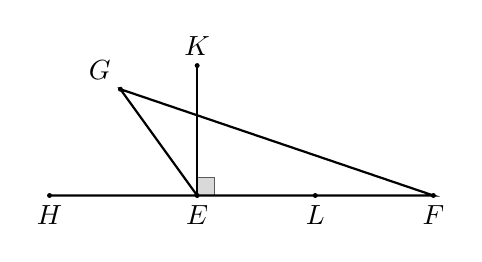
\begin{tikzpicture}[scale=0.75]
  \coordinate (H) at (-2.5,0); \coordinate (E) at (0,0); \coordinate (L) at (2,0);
  \coordinate (F) at (4,0); \coordinate (G) at (-1.3,1.8); \coordinate (K) at (0,2.2);
  \draw[gray!70!black, fill=gray!30] (E) rectangle ++(0.3,0.3);
  \draw[thick] (H) -- (F) -- (G) -- (E); \draw[thick] (E) -- (K);
  \foreach \p in {H,E,L,F,G,K} \fill (\p) circle (1.2pt);
  \node[below] at (H) {$H$}; \node[below] at (E) {$E$}; \node[below] at (L) {$L$};
  \node[below] at (F) {$F$}; \node[above left] at (G) {$G$}; \node[above] at (K) {$K$};
\end{tikzpicture}
\end{minipage}%
\hfill
\begin{minipage}[c]{0.64\linewidth}
Les points $H$, $E$, $L$ et $F$ sont alignés. Complète.

\renewcommand{\arraystretch}{1.5}
\begin{tabular}{@{}ll@{}}
\textit{Exemple :} $\widehat{GEF}$ est un angle obtus. & $\widehat{HEF}$ est un angle \rep[1.4cm]{plat}. \\
$\widehat{EFG}$ est un angle \rep[1.4cm]{aigu}. & $\widehat{KEF}$ est un angle \rep[1.4cm]{droit}. \\
$\widehat{HEG}$ est un angle \rep[1.4cm]{aigu}. & $\widehat{LEF}$ est un angle \rep[1.4cm]{nul}. \\
\end{tabular}
\end{minipage}
\end{exercicedevoir}

\vspace{-1.1cm}
\begin{exercicedevoir}[3][Vrai ou faux ?]
\vspace{-0.3cm}
Entoure la bonne réponse.

\renewcommand{\arraystretch}{1.2}
\begin{tabular}{@{}l@{\qquad}l@{}}
a) Un angle de $150^\circ$ est un angle obtus. & \vf{1} \\
b) Un angle plat mesure $90^\circ$. & \vf{2} \\
c) Un angle aigu peut mesurer $95^\circ$. & \vf{2} \\
\end{tabular}
\end{exercicedevoir}

\vspace{-0.6cm}

\newpage
\bandeau[]{6C04-GEO13}{Classer des angles selon leur nature}
\vspace{-0.5cm}


% ------------------------------------------------------------------
% Panneau : mesures réelles (différentes de la fiche Ex-6C04-04 et du QCM)
%  ABC  50 aigu (exemple) | DEF  90 droit | GHI 150 obtus | JKL  30 aigu
%  MNP 180 plat           | RST 115 obtus | UVW  90 droit | XYZ  70 aigu
%  EOF 130 obtus          | TAU  25 aigu
% Bilan : 4 aigus (dont l'exemple), 2 droits, 3 obtus, 1 plat.
% ------------------------------------------------------------------
\begin{exercicedevoir}[9][Classe les angles]
\vspace{-0.3cm}
Écris le nom de chaque angle dans la bonne colonne du tableau, comme dans l'exemple.

\smallskip
\centering
\setlength{\tabcolsep}{2pt}
\fbox{\begin{tabular}{@{}ccccc@{}}
\caseAngle{50}{140}{A}{B}{C} & \caseAngle{90}{75}{D}{E}{F} &
\caseAngle{150}{15}{G}{H}{I} & \caseAngle{30}{200}{J}{K}{L} &
\caseAngle{180}{120}{M}{N}{P} \\[1mm]
\caseAngle{115}{280}{R}{S}{T} & \caseAngle{90}{345}{U}{V}{W} &
\caseAngle{70}{30}{X}{Y}{Z} & \caseAngle{130}{230}{E}{O}{F} &
\caseAngle{25}{75}{T}{A}{U} \\
\end{tabular}}

\medskip
\renewcommand{\arraystretch}{1.3}
\begin{tabularx}{\linewidth}{|*{4}{>{\centering\arraybackslash}X|}}
\hline
\textbf{Angles aigus} & \textbf{Angles droits} & \textbf{Angles obtus} & \textbf{Angles plats} \\ \hline
\casetab{1.1cm}{\textit{Exemple :} $\widehat{ABC}$ \ \cor{$\widehat{JKL}$ \ $\widehat{XYZ}$ \ $\widehat{TAU}$}} &
\casetab{1.1cm}{\cor{$\widehat{DEF}$ \ $\widehat{UVW}$}} &
\casetab{1.1cm}{\cor{$\widehat{GHI}$ \ $\widehat{RST}$ \ $\widehat{EOF}$}} &
\casetab{1.1cm}{\cor{$\widehat{MNP}$}} \\ \hline
\end{tabularx}
\end{exercicedevoir}

% Mesures : nul 0 ; aigus 30 (ex.), 88 ; droit 90 ; obtus 95, 160 ; plat 180.
\vspace{-1.1cm}
\begin{exercicedevoir}[6][Classe les mesures]
\vspace{-0.3cm}
Range chaque mesure dans la bonne colonne, comme dans l'exemple.

\smallskip
\centering
\textit{Exemple :} $30\degre$ \qquad\qquad $95\degre$ \qquad $0\degre$ \qquad $88\degre$ \qquad $180\degre$ \qquad $160\degre$ \qquad $90\degre$

\medskip
\renewcommand{\arraystretch}{1.3}
\begin{tabularx}{\linewidth}{|*{5}{>{\centering\arraybackslash}X|}}
\hline
\textbf{Nul} & \textbf{Aigu} & \textbf{Droit} & \textbf{Obtus} & \textbf{Plat} \\ \hline
\casetab{0.8cm}{\cor{$0\degre$}} &
\casetab{0.8cm}{\textit{Ex. :} $30\degre$ \ \cor{$88\degre$}} &
\casetab{0.8cm}{\cor{$90\degre$}} &
\casetab{0.8cm}{\cor{$95\degre$ \ $160\degre$}} &
\casetab{0.8cm}{\cor{$180\degre$}} \\ \hline
\end{tabularx}
\end{exercicedevoir}

\vspace{-1.1cm}
\begin{exercicedevoir}[5][Pour aller plus loin]
\vspace{-0.3cm}
\textbf{1.} Range ces angles du panneau du \textbf{plus petit} au \textbf{plus grand}. \hfill \textit{(2 points)}

\smallskip
$\widehat{MNP}$, \ $\widehat{TAU}$, \ $\widehat{DEF}$, \ $\widehat{GHI}$ \qquad $\longrightarrow$ \qquad
\repB[1.4cm]{$\widehat{TAU}$} $<$ \repB[1.4cm]{$\widehat{DEF}$} $<$ \repB[1.4cm]{$\widehat{GHI}$} $<$ \repB[1.4cm]{$\widehat{MNP}$}

\medskip
\textbf{2.} Entoure \textbf{toutes} les mesures d'angles \textbf{aigus}. \hfill \textit{(3 points)}

\smallskip
\centering
\entoure[r]{$45\degre$} \quad \entoure{$100\degre$} \quad \entoure[r]{$89\degre$} \quad \entoure{$90\degre$} \quad \entoure[r]{$3\degre$} \quad \entoure{$170\degre$} \quad \entoure[r]{$60\degre$} \quad \entoure{$0\degre$} \quad \entoure{$180\degre$}
\end{exercicedevoir}

\vspace{-0.6cm}
}

\begin{document}

\corrigefalse
\feuille

\end{document}

%%% Local Variables:
%%% mode: LaTeX
%%% TeX-master: t
%%% End:
